%% abtex2-modelo-trabalho-academico.tex, v-1.9.6 laurocesar
%% Copyright 2012-2016 by abnTeX2 group at http://www.abntex.net.br/ 
%%
%% This work may be distributed and/or modified under the
%% conditions of the LaTeX Project Public License, either version 1.3
%% of this license or (at your option) any later version.
%% The latest version of this license is in
%%   http://www.latex-project.org/lppl.txt
%% and version 1.3 or later is part of all distributions of LaTeX
%% version 2005/12/01 or later.
%%
%% This work has the LPPL maintenance status `maintained'.
%% 
%% The Current Maintainer of this work is the abnTeX2 team, led
%% by Lauro César Araujo. Further information are available on 
%% http://www.abntex.net.br/
%%
%% This work consists of the files abntex2-modelo-trabalho-academico.tex,
%% abntex2-modelo-include-comandos and abntex2-modelo-references.bib
%%

% ------------------------------------------------------------------------
% ------------------------------------------------------------------------
% abnTeX2: Modelo de Trabalho Academico (tese de doutorado, dissertacao de
% mestrado e trabalhos monograficos em geral) em conformidade com 
% ABNT NBR 14724:2011: Informacao e documentacao - Trabalhos academicos -
% Apresentacao
% ------------------------------------------------------------------------
% ------------------------------------------------------------------------

\documentclass[
	% -- opções da classe memoir --
	12pt,				% tamanho da fonte
	%openright,			% capítulos começam em pág ímpar (insere página vazia caso preciso)
	%twoside,			% para impressão em recto e verso. Oposto a oneside
	oneside,			% impressão de um lado só
	a4paper,			% tamanho do papel. 
	% -- opções da classe abntex2 --
	chapter=TITLE,		% títulos de capítulos convertidos em letras maiúsculas
	section=TITLE,		% títulos de seções convertidos em letras maiúsculas
	%subsection=TITLE,	% títulos de subseções convertidos em letras maiúsculas
	%subsubsection=TITLE,% títulos de subsubseções convertidos em letras maiúsculas
	sumario=tradicional % opção de sumário
	% -- opções do pacote babel --
	english,			% idioma adicional para hifenização
	french,				% idioma adicional para hifenização
	spanish,			% idioma adicional para hifenização
	brazil				% o último idioma é o principal do documento
	]{abntex2}

% ---
% Pacotes básicos 
% ---
\usepackage{lmodern}			% Usa a fonte Latin Modern			
\usepackage[T1]{fontenc}		% Selecao de codigos de fonte.
\usepackage[utf8]{inputenc}		% Codificacao do documento (conversão automática dos acentos)
\usepackage{lastpage}			% Usado pela Ficha catalográfica
\usepackage{indentfirst}		% Indenta o primeiro parágrafo de cada seção.
\usepackage{color}				% Controle das cores
\usepackage{graphicx}			% Inclusão de gráficos
\usepackage{microtype} 			% Melhorias de justificação
\usepackage{hyperref}
\usepackage{facens}				% Padrão Facens
\usepackage{pdfpages}			% Include de pdfs
\usepackage{lipsum}				% Geração de dummy text
\usepackage[alf]{abntex2cite}	% Citações padrão ABNT
%\usepackage[brazilian,hyperpageref]{backref}	 % Paginas com as citações na bibl
% ---

% ---
% Indicando pasta de figuras\\
% ---
\graphicspath{{imagens/}}
% ---

% --- 
% CONFIGURAÇÕES DE PACOTES
% --- 

% ---
% Configurações do pacote backref
% Usado sem a opção hyperpageref de backref
%\renewcommand{\backrefpagesname}{Citado na(s) página(s):~}
% Texto padrão antes do número das páginas
%\renewcommand{\backref}{}
% Define os textos da citação
%\renewcommand*{\backrefalt}[4]{
%	\ifcase #1 %
%		Nenhuma citação no texto.%
%	\or
%		Citado na página #2.%
%	\else
%		Citado #1 vezes nas páginas #2.%
%	\fi}%
% ---

%VARIAVEIS
%---

%---
% ---
% Informações de dados para CAPA e FOLHA DE ROSTO
% ---
\titulo{RELATÓRIO DE ESTÁGIO SUPERVISIONADO OBRIGATÓRIO}
\autor{Alex Covolan Vieira Coelho}
\local{Sorocaba/SP}
\data{2017}
\orientador[Dra.]{Andrea Vieira Braga}
\instituicao{Faculdade de Engenharia de Sorocaba - FACENS}
\tipotrabalho{Dissertação}

% O preambulo deve conter o tipo do trabalho, o objetivo, 
% o nome da instituição e a área de concentração 
\preambulo{Relatório apresentado como requisito obrigatório para a integralização do Curso de Engenharia da Computação.}
% ---


% ---
% Configurações de aparência do PDF final

% alterando o aspecto da cor azul
\definecolor{blue}{RGB}{41,5,195}

% informações do PDF
\makeatletter
\hypersetup{
     	%pagebackref=true,
		pdftitle={\@title}, 
		pdfauthor={\@author},
    	pdfsubject={\imprimirpreambulo},
	    pdfcreator={LaTeX with abnTeX2},
		pdfkeywords={abnt}{latex}{abntex}{abntex2}{trabalho acadêmico}, 
		colorlinks=false,       		% false: boxed links; true: colored links
    	linkcolor=blue,          	% color of internal links
    	citecolor=blue,        		% color of links to bibliography
    	filecolor=magenta,      		% color of file links
		urlcolor=blue,
		bookmarksdepth=4
}
\makeatother
% --- 

% --- 
% Espaçamentos entre linhas e parágrafos 
% --- 

% O tamanho do parágrafo é dado por:
\setlength{\parindent}{1.25cm}

% Controle do espaçamento entre um parágrafo e outro:
\setlength{\parskip}{0.2cm}  % tente também \onelineskip

% ---
% compila o indice
% ---
\makeindex
% ---

% ----
% Início do documento
% ----
\begin{document}
% Seleciona o idioma do documento (conforme pacotes do babel)
%\selectlanguage{english}
\selectlanguage{brazil}

% Retira espaço extra obsoleto entre as frases.
\frenchspacing 

% ----------------------------------------------------------
% ELEMENTOS PRÉ-TEXTUAIS
% ----------------------------------------------------------
\pretextual

%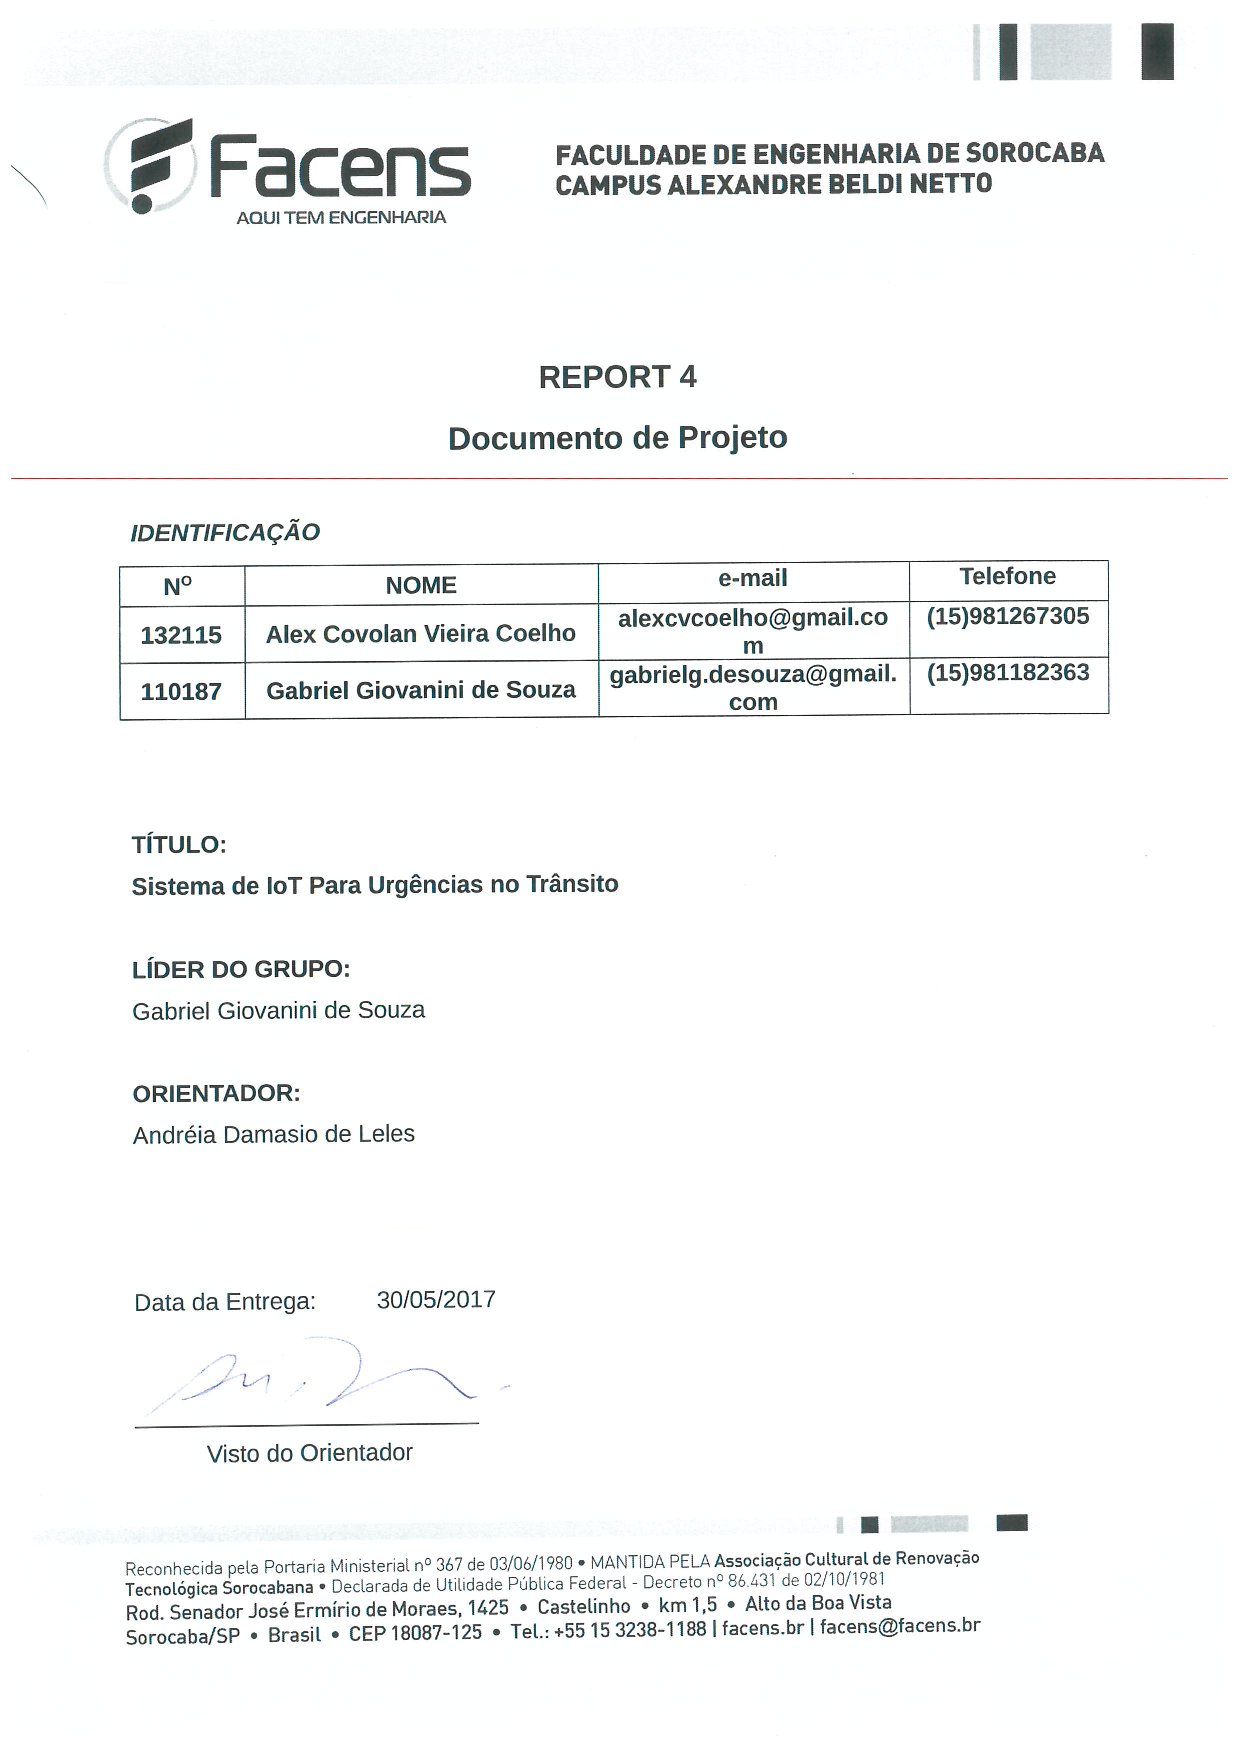
\includepdf{report4.pdf}


% ---
% Capa
% ---
\imprimircapa
% ---

% ---
% Folha de rosto
% (o * indica que haverá a ficha bibliográfica)
% ---
\imprimirfolhaderosto*
% ---

% ---
% Inserir a ficha bibliografica
% ---

% Isto é um exemplo de Ficha Catalográfica, ou ``Dados internacionais de
% catalogação-na-publicação''. Você pode utilizar este modelo como referência. 
% Porém, provavelmente a biblioteca da sua universidade lhe fornecerá um PDF
% com a ficha catalográfica definitiva após a defesa do trabalho. Quando estiver
% com o documento, salve-o como PDF no diretório do seu projeto e substitua todo
% o conteúdo de implementação deste arquivo pelo comando abaixo:
%
% \begin{fichacatalografica}
%     \includepdf{fig_ficha_catalografica.pdf}
% \end{fichacatalografica}

%\begin{fichacatalografica}
	\sffamily
	\vspace*{\fill}					% Posição vertical
	\begin{center}					% Minipage Centralizado
	\fbox{\begin{minipage}[c][8cm]{13.5cm}		% Largura
	\small
	\imprimirautor
	%Sobrenome, Nome do autor
	
	\hspace{0.5cm} \imprimirtitulo  / \imprimirautor. --
	\imprimirlocal, \imprimirdata-
	
	\hspace{0.5cm} \pageref{LastPage} p. : il. (algumas color.) ; 30 cm.\\
	
	\hspace{0.5cm} \imprimirorientadorRotulo~\imprimirorientador\\
	
	\hspace{0.5cm}
	\parbox[t]{\textwidth}{\imprimirtipotrabalho~--~\imprimirinstituicao,
	\imprimirdata.}\\
	
	\hspace{0.5cm}
		1. Palavra-chave1.
		2. Palavra-chave2.
		2. Palavra-chave3.
		I. Orientador.
		II. Universidade xxx.
		III. Faculdade de xxx.
		IV. Título 			
	\end{minipage}}
	\end{center}
\end{fichacatalografica}
% ---

% ---
% Inserir errata
% ---
%\begin{errata}
Elemento opcional da \citeonline[4.2.1.2]{NBR14724:2011}. Exemplo:

\vspace{\onelineskip}

FERRIGNO, C. R. A. \textbf{Tratamento de neoplasias ósseas apendiculares com
reimplantação de enxerto ósseo autólogo autoclavado associado ao plasma
rico em plaquetas}: estudo crítico na cirurgia de preservação de membro em
cães. 2011. 128 f. Tese (Livre-Docência) - Faculdade de Medicina Veterinária e
Zootecnia, Universidade de São Paulo, São Paulo, 2011.

\begin{table}[htb]
\center
\footnotesize
\begin{tabular}{|p{1.4cm}|p{1cm}|p{3cm}|p{3cm}|}
  \hline
   \textbf{Folha} & \textbf{Linha}  & \textbf{Onde se lê}  & \textbf{Leia-se}  \\
    \hline
    1 & 10 & auto-conclavo & autoconclavo\\
   \hline
\end{tabular}
\end{table}

\end{errata}
% ---

% ---
% Inserir folha de aprovação
% ---

% Isto é um exemplo de Folha de aprovação, elemento obrigatório da NBR
% 14724/2011 (seção 4.2.1.3). Você pode utilizar este modelo até a aprovação
% do trabalho. Após isso, substitua todo o conteúdo deste arquivo por uma
% imagem da página assinada pela banca com o comando abaixo:
%
% \includepdf{folhadeaprovacao_final.pdf}
%
%\begin{folhadeaprovacao}

  \begin{center}
    {\ABNTEXchapterfont\large\imprimirautor}

    \vspace*{\fill}\vspace*{\fill}
    \begin{center}
      \ABNTEXchapterfont\bfseries\Large\imprimirtitulo
    \end{center}
    \vspace*{\fill}
    
    \hspace{.45\textwidth}
    \begin{minipage}{.5\textwidth}
        \imprimirpreambulo
    \end{minipage}%
    \vspace*{\fill}
   \end{center}
        
   Trabalho aprovado. \imprimirlocal, 24 de novembro de 2012:

   \assinatura{\textbf{\imprimirorientador} \\ Orientador} 
   \assinatura{\textbf{Professor} \\ Convidado 1}
   \assinatura{\textbf{Professor} \\ Convidado 2}
   %\assinatura{\textbf{Professor} \\ Convidado 3}
   %\assinatura{\textbf{Professor} \\ Convidado 4}
      
   \begin{center}
    \vspace*{0.5cm}
    {\large\imprimirlocal}
    \par
    {\large\imprimirdata}
    \vspace*{1cm}
  \end{center}
  
\end{folhadeaprovacao}
% ---

% ---
% Dedicatória
% ---
%\begin{dedicatoria}
   \vspace*{\fill}
   \centering
   \noindent
   \textit{ Este trabalho é dedicado às crianças adultas que,\\
   quando pequenas, sonharam em se tornar cientistas.} \vspace*{\fill}
\end{dedicatoria}
% ---

% ---
% Agradecimentos
% ---
%\begin{agradecimentos}
Os agradecimentos principais são direcionados à Gerald Weber, Miguel Frasson,
Leslie H. Watter, Bruno Parente Lima, Flávio de Vasconcellos Corrêa, Otavio Real
Salvador, Renato Machnievscz\footnote{Os nomes dos integrantes do primeiro
projeto abn\TeX\ foram extraídos de
\url{http://codigolivre.org.br/projects/abntex/}} e todos aqueles que
contribuíram para que a produção de trabalhos acadêmicos conforme
as normas ABNT com \LaTeX\ fosse possível.

Agradecimentos especiais são direcionados ao Centro de Pesquisa em Arquitetura
da Informação\footnote{\url{http://www.cpai.unb.br/}} da Universidade de
Brasília (CPAI), ao grupo de usuários
\emph{latex-br}\footnote{\url{http://groups.google.com/group/latex-br}} e aos
novos voluntários do grupo
\emph{\abnTeX}\footnote{\url{http://groups.google.com/group/abntex2} e
\url{http://www.abntex.net.br/}}~que contribuíram e que ainda
contribuirão para a evolução do \abnTeX.

\end{agradecimentos}
% ---

% ---
% Epígrafe
% ---
%\begin{epigrafe}
    \vspace*{\fill}
	\begin{flushright}
		\textit{``Não vos amoldeis às estruturas deste mundo, \\
		mas transformai-vos pela renovação da mente, \\
		a fim de distinguir qual é a vontade de Deus: \\
		o que é bom, o que Lhe é agradável, o que é perfeito.\\
		(Bíblia Sagrada, Romanos 12, 2)}
	\end{flushright}
\end{epigrafe}
% ---

% ---
% RESUMOS
% ---

% resumo em português
%\setlength{\absparsep}{18pt} % ajusta o espaçamento dos parágrafos do resumo
\begin{resumo}
 Segundo a \citeonline[3.1-3.2]{NBR6028:2003}, o resumo deve ressaltar o
 objetivo, o método, os resultados e as conclusões do documento. A ordem e a extensão
 destes itens dependem do tipo de resumo (informativo ou indicativo) e do
 tratamento que cada item recebe no documento original. O resumo deve ser
 precedido da referência do documento, com exceção do resumo inserido no
 próprio documento. (\ldots) As palavras-chave devem figurar logo abaixo do
 resumo, antecedidas da expressão Palavras-chave:, separadas entre si por
 ponto e finalizadas também por ponto.

 \textbf{Palavras-chave}: latex. abntex. editoração de texto.
\end{resumo}

% resumo em inglês
%\begin{resumo}[Abstract]
 \begin{otherlanguage*}{english}
   This is the english abstract.

   \vspace{\onelineskip}
 
   \noindent 
   \textbf{Keywords}: latex. abntex. text editoration.
 \end{otherlanguage*}
\end{resumo}

% ---

% ---
% inserir lista de ilustrações
% ---
\pdfbookmark[0]{\listfigurename}{lof}
\listoffigures*
\cleardoublepage
% ---

% ---
% inserir lista de tabelas
% ---
%\pdfbookmark[0]{\listtablename}{lot}
\listoftables*
\cleardoublepage
% ---

% ---
% inserir lista de abreviaturas e siglas
% ---
\begin{siglas}
  \item[CRTSE] Centro Regional de Tecnologia Santa Escolástica
  \item[CRTS] Companhia Rede Telefônica Sorocabana
  \item[ACRTS] Associação Cultural de Renovação Tecnológica Sorocabana
  \item[IPEAS] Instituto de Pesquisas e Estudos Avançados Sorocabano
  \item[LEMAT] Laboratório de Ensaio de Materiais
  \item[ABMES] Associação Brasileira de Mantenedoras de Ensino Superior
\end{siglas}
% ---

% ---
% inserir lista de símbolos
% ---
%\begin{simbolos}
  \item[$ \Gamma $] Letra grega Gama
  \item[$ \Lambda $] Lambda
  \item[$ \zeta $] Letra grega minúscula zeta
  \item[$ \in $] Pertence
\end{simbolos}
% ---

% ---
% inserir o sumario
% ---
\pdfbookmark[0]{\contentsname}{toc}
\tableofcontents*
\cleardoublepage
% ---



% ----------------------------------------------------------
% ELEMENTOS TEXTUAIS
% ----------------------------------------------------------
\textual
% ---
\pagestyle{simple}


\chapter{Introdução}
\label{chap:cap1}
O presente relatório de estágio é elaborado como documento obrigatório para a conclusão do curso de Engenharia da Computação, apresentando as atividades realizadas durante as 360 horas de estágio, cumpridas dentro da Faculdade de Engenharia de Sorocaba (Facens). Mais especificamente atuando dentro do Laboratório de Informática, nos primeiros meses trabalhando com suporte aos computadores presentes na faculdade, além de atendimento \textit{help desk} e posteriormente trabalhando com desenvolvimento de aplicações WEB em PHP as quais serviram para atender as demandas da própria faculdade, tanto no âmbito corporativo como no educacional.

Tal estágio também proporcionou uma posterior contratação ao término dos 2 anos previsto em contrato, e este é o período considerado neste documento, pois após a contratação as áreas de atuação foram ampliadas, garantindo sólidos conhecimentos em novas tecnologias e plataformas, como Ruby, C\# e a plataforma Sales Force, compreendendo o período de maior aprendizado durante esta jornada. 

Mesmo com as novas tecnologias e áreas de atuação, a maior parte das aplicações a serem criadas continuaram sendo em PHP, além de dar suporte as aplicações antigas. Foi possível também aprender sobre a área de infraestrutura, passando a desempenhar a função de \textit{devops} e trabalhando ao lado dos analistas de redes.

Dentre os feitos durante o estágio, destaca-se a doação de um sistema de inscrições para a FUNDEC (Fundação de Desenvolvimento Cultural de Sorocaba), tal sistema agilizou a inscrição e processo de seleção de mais de 4 mil candidatos, os quais eram cadastrados na mão anteriormente, também é possível enunciar a colaboração no desenvolvimento de uma \textit{framework} própria desenvolvida dentro da FACENS pelo Eng. Flávio Bogila a qual ganhou o nome de "Bogila Framework", através dela possibilitou-se criar novas aplicações com maior velocidade devido ao fato dela já possuir \textit{templates} padrões, geração de código e uma arquitetura que facilitam seu uso nas aplicações da Faculdade.

\chapter{Plano de Estágio}
\label{chap:cap2}
Informações sobre a empresa e o estagiário são apresentados nesta seção.
\section{Identificação do Aluno}
\label{sec:identaluno}
\textbf{Nome:} Alex Covolan Vieira Coelho\\
\indent \textbf{Matrícula: } 132115\\
\indent \textbf{Curso: } Engenharia da Computação\\
\indent \textbf{Semestre: } 10º\\
\indent \textbf{Ano de ingresso: } 2013\\
\indent \textbf{E-mail: } alexcvcoelho@gmail.com\\

\section{Empresa}
\label{sec:empresa}
\textbf{Nome:} FACENS - Faculdade de Engenharia de Sorocaba \\
\indent \textbf{Razão Social:} Associacao Cultural de Renovacao Tecnologica Sorocabana \\
\indent \textbf{CNPJ:} 45.718.988/0003-29 \\
\indent \textbf{Área de atuação:} Educação superior\\
\indent \textbf{Endereço:} Rodovia Senador José Ermírio de Moraes, 1425 \\
\indent \textbf{Bairro:} Castelinho km 1,5 - Alto da Boa Vista \\
\indent \textbf{CEP:} 18087-125 \\
\indent \textbf{Cidade:} Sorocaba \\
\indent \textbf{Estado:} São Paulo \\
\indent \textbf{Nome do responsável pelos estágios na empresa:} João Alex Ramon \\
\indent \textbf{Telefone da área responsável pelos estágios:} (15) 3238-1188/216 \\

\begin{figure}[htb]
\caption{\label{fig:mapsfacens} Localização da Facens}
\begin{center}
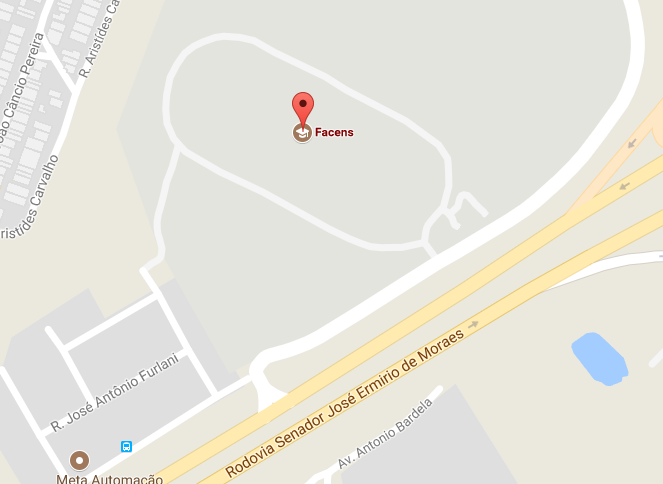
\includegraphics[scale=0.65]{MapsFacens}
\end{center}
\end{figure}

\section{Estágio}
\label{sec:estagio}
\textbf{Área de atuação:} Desenvolvimento \\
\indent \textbf{Setor:} Tecnologia da Informação \\
\indent \textbf{Data de início de estágio:} \\
\indent \textbf{Data do fim de estágio:} \\
\indent \textbf{Período do dia que estagia:} Manhã e Tarde \\
\indent \textbf{Carga horária semanal:} 40 horas \\

\section{Supervisor de Estágio na Empresa}
\label{sec:supestagioempre}
\textbf{Nome:} Luis Gustavo Martins Monteiro \\
\indent \textbf{Formação acadêmica:} \\
\indent \indent Especialização em Redes de Computadores, UNICAMP, 2006 \\
\indent \indent Graduação em Sistemas de Informação, Uirapuru Superior, 2005 \\
\indent \textbf{Cargo:} Coordenador da Tecnologia da Informação \\
\indent \textbf{Departamento:} Tecnologia da Informação \\
\indent \textbf{Responsabilidades do departamento:} Desenvolvimento e suporte de soluções tecnológicas \\
\indent \textbf{Telefone:} (15) 3238-1188/236 \\
\indent \textbf{E-mail:} gustavo.monteiro@facens.br \\

\section{Atividades Programadas Para o Estagiário}
\label{sec:ativestagiario}


\chapter{Organograma da Empresa}
\label{chap:chap3}
\textbf{Diretor:} \\ \indent Eng. Paulo Roberto Freitas de Carvalho \\
\indent paulo.carvalho@facens.br \\

\textbf{Vice Diretor:} \\ \indent  Prof. Dr. Fabiano Prado Marques \\
\indent fabiano.marques@facens.br \\

\textbf{Coordenação Engenharia Civil:}\\ \indent  Prof. Dr. José Antonio De Milito \\
\indent jose.milito@facens.br \\

\textbf{Coordenação Engenharia da Computação:}\\ \indent Prof.ª Dra. Andréa Lucia Braga Vieira Rodrigues \\
\indent andrea.braga@facens.br \\

\textbf{Coordenação Engenharia Elétrica:} \\ \indent Prof. Dr. Anderson Marcos Henriques \\
\indent anderson.henriques@facens.br \\

\textbf{Coordenação Engenharia Mecânica:} \\ \indent Prof. Dr. Francisco Scinocca \\
\indent francisco.scinocca@facens.br \\

\textbf{Coordenação Engenharia Mecatrônica:} \\ \indent Prof. Dr. Anderson Marcos Henriques \\
\indent anderson.henriques@facens.br \\

\textbf{Coordenação Engenharia Produção:} \\ \indent Prof. Dr. José Lázaro Ferraz \\
\indent jose.ferraz@facens.br \\

\textbf{Coordenação Engenharia Química:} \\ \indent Prof.ª Dra. Sandra Bizarria Lopes Villanueva \\
\indent sandra.lopes@facens.br \\

\textbf{Coordenação Tecnologia em Jogos Digitais:} \\ \indent Prof.ª Dra. Andréa Lucia Braga Vieira Rodrigues \\
\indent andrea.braga@facens.br \\

\textbf{Coordenação Engenharia Agronômica:} \\ \indent Prof.ª Me. Thais Prado Avancini \\
\indent thais.avancini@facens.br \\

\textbf{Coordenação Engenharia de Alimentos:} \\ \indent Prof. Dra. Cláudia Maria Treumann Rocha \\
\indent claudia.treumann@facens.br \\

\textbf{Coordenação Acadêmica:} \\ \indent Prof.ª Dra. Sandra Bizarria Lopes Villanueva \\
\indent sandra.lopes@facens.br \\

\textbf{Coordenação Ciclo Básico:} \\ \indent Prof. Me. Marcos Vinícius Ribeiro \\
\indent marcos.ribeiro@facens.br \\

\textbf{Coordenação de projetos:}  \\

\textbf{Smart Campus Facens:} \\ \indent Prof.ª Dra. Regiane Relva Romano \\
\indent regiane.relva@facens.br \\

\textbf{Fab Lab Facens:} \\ \indent Siron Cesar Paccheco Pereira \\
\indent siron.pereira@facens.br \\

\textbf{LIGA Facens:} \\ \indent Prof. Wilson Roberto Marcondes de Oliveira Junior \\
\indent wilson.junior@facens.br \\

\textbf{Pós, Extensão e Cursinho Pré-Vestibular:} \\ \indent Prof. Dr. Adriano Pila \\
\indent adriano.pila@facens.br \\

\textbf{Facens Tech (IPEAS/LEMAT/LIGA):} \\ \indent Prof. Me. Antonio Carlos Gomes \\
\indent antonio.gomes@facens.br \\

\textbf{Farm Lab Facens:} \\ \indent Prof.ª Me. Thais Prado Avancini \\
\indent thais.avancini@facens.br \\

\textbf{FACE (Facens Centro de Empreendedorismo):} \\ \indent Prof.ª Me. Andréia Damasio Leles \\
\indent andrea.leles@facens.br

\section{A Empresa}
\label{sec:aempresa}
\begin{figure}[htb]
	\caption{\label{fig:mapsfacens} Faixada da Facens}
	\begin{center}
		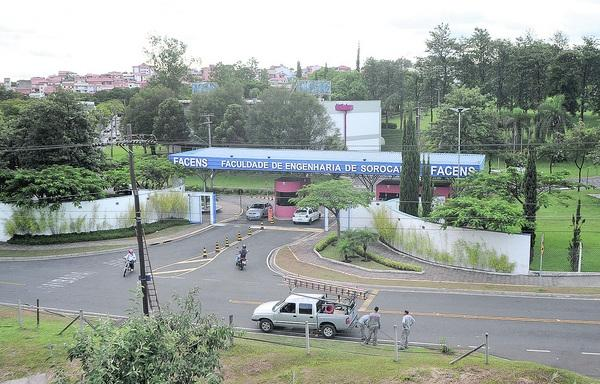
\includegraphics[scale=0.85]{facensfachada}
	\end{center}
\end{figure}

A Faculdade de Engenharia de Sorocaba - Facens - teve como embrião a Companhia Rede Telefônica Sorocabana ( CRTS ) responsável pelo sistema de telefonia de toda região sorocabana, em meados dos anos 70. A necessidade de profissionais capacitados para atuar no setor de telecomunicações fez com que a CRTS criasse, em 1974, o Centro Regional de Tecnologia Santa Escolástica ( CRTSE ), mais conhecido como Colégio da Engenharia. Os cursos de Telecomunicações e Eletrônica foram os primeiros a ser ministrados pelo colégio técnico - em salas cedidas pelo Colégio Santa Escolástica.

O rápido desenvolvimento do setor de telecomunicações na região fez com que a mão de obra especializada se tornasse imprescindível. No mesmo ano de implantação do Colégio, a Associação Cultural de Renovação Tecnológica Sorocabana (ACRTS) - mantenedora do Colégio da Engenharia e da Facens - protocolou no Ministério de Educação e Cultura (MEC) um pedido para instalação da Faculdade de Engenharia na cidade de Sorocaba. Em outubro de 1976, foi publicada a autorização para a implantação dos primeiros cursos da Faculdade, de Engenharia Civil e Engenharia Elétrica os quais tiveram seus vestibulares abertos em janeiro de 1977, que passaram a funcionar no 3º andar do Instituto de Educação Ciências e Letras.

Em 1978, foram iniciadas as construções do campus universitário da Faculdade criada para suprir uma grave lacuna no Ensino Superior de Sorocaba. Em 03 de junho de 1980, a Facens foi reconhecida pelo MEC. A construção do campus foi concluída em 1984 com a implantação dos prédios de Engenharia Civil e Elétrica, laboratórios para esses cursos e o ginásio de esportes.
Em anos mais recentes, a Facens recebeu autorização para ministrar os cursos de Engenharia da Computação (1998) e de Engenharia Mecânica (2001) atendendo assim, à crescente demanda por tais profissionais na Região. Por este mesmo motivo passou a oferecer, no final da década de 90, cursos de Especialização e Pós-Graduação Lato-Sensu.

Em 1991 a Semana da Engenharia foi incluída no calendário acadêmico, passando a expor projetos de alunos durante três dias a todos da comunidade, além de proporcionar cursos e palestras para os alunos. Em 2001 a Facens passou a oferecer o curso de Engenharia Mecânica reconhecido pelo MEC, a fim de capacitar profissionais para o Parque Tecnológico da região. No mesmo ano o IPEAS (Instituto de Pesquisas e Estudos Avançados Sorocabano) começou suas atividades dentro do campus, prestando serviços a empresas da região na área tecnológica. Em 2003 o LEMAT (Laboratório de Ensaio de Materiais) deixou de atuar apenas como laboratório acadêmico, passando a prestar serviços para empresas da região.

Em 2004 iniciou-se o Cursinho Pré-Vestibular com a intenção de nivelar o conhecimento de alunos da rede pública e privada para ingresso nas instituições de ensino superior. Em 2005 foi realizada a 1ª Maratona de Programação O evento é uma competição interna que a faculdade promove seguindo os moldes da Maratona de Programação da Sociedade Brasileira de Computação (Regional Sulamericana do Concurso da ACM). A maratona é um torneio onde equipes formadas por alunos devem resolver problemas computacionais, utilizando conhecimentos técnicos, criatividade, capacidade de trabalho em equipe e habilidade de resolver problemas sob pressão.

Em 2008 é realizada a 1ª Maratona de Desenvolvimento de Jogos. A Maratona de Desenvolvimento de Jogos da Facens é um concurso técnico e cultural que busca incentivar o estudo e a aplicação das tecnologias que envolvem o desenvolvimento de jogos eletrônicos por parte dos alunos da Faculdade.

Em 2010 é aberto o curso de Engenharia Mecatrônica. Em 2011 é dado início a Construção do Prédio C. Nos 7 mil metros quadrados de construção são mais 30 salas de aula, todas equipadas com lousas digitais, sistema de som e adequações acústicas. Com estrutura pré-montada e linhas arquitetônicas modernas, além de utilizar toda a tecnologia disponível, existe também a preocupação com sustentabilidade.

\begin{figure}[htb]
	\caption{\label{fig:mapsfacens} Prédio C}
	\begin{center}
		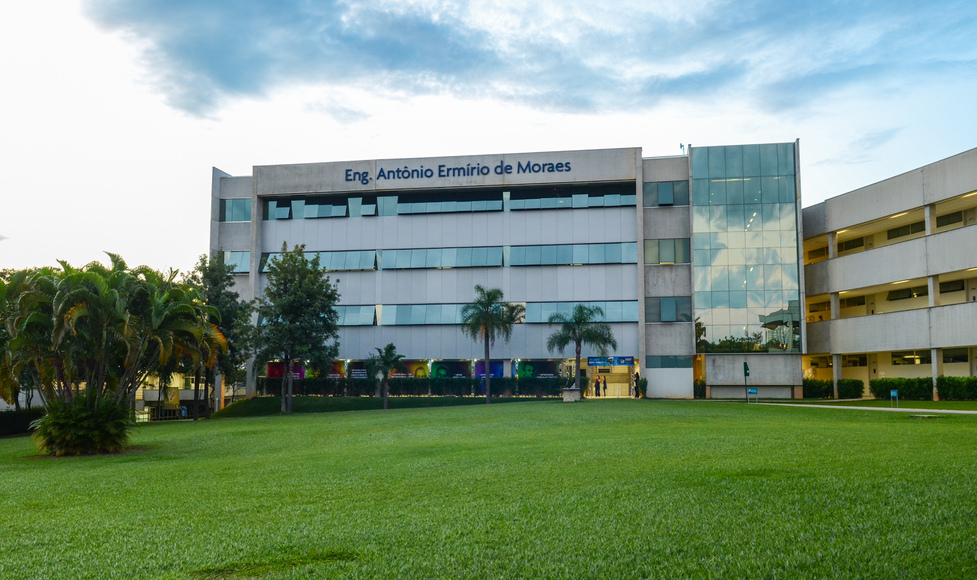
\includegraphics[scale=0.85]{predioc}
	\end{center}
\end{figure}

Em 2012 é aberto o curso de Engenharia de Produção e Engenharia Química. Em 2014 é lançado o Smart Campus Facens com o objetivo de  desenvolver, implementar, testar, analisar e replicar soluções para Cidades Inteligentes, utilizando o campus universitário como uma área para estudos das soluções que possam ser replicadas nas cidades. Prioriza-se a transformação de problemas reais em soluções aplicáveis no contexto urbano, alinhando-as com as necessidades, crises e desafios do Brasil para as próximas décadas. 

Em 2015 iniciou-se o curso de Tecnologia de Jogos Digitais, o primeiro curso tecnólogo dentro da Facens. No mesmo ano ocorreu a inauguração do Fab Lab Facens, o primeiro laboratório de prototipação no interior de São Paulo, o Fab Lab Facens é um laboratório de fabricação digital pertencente à rede mundial Fab Lab, criada pelo MIT com o objetivo de facilitar a prototipagem de ideias e visando a inovação e invenção. Onde estudantes, educadores, empresas, profissionais, inventores, curiosos e especialistas podem adquirir conhecimento, trocar experiências e utilizar equipamentos para tornar seus projetos em realidade.

Em 2016 iniciou-se o curso de Engenharia de Alimentos e Engenharia Agronômica. No mesmo ano a Facens ganhou o Prêmio Top Educacional através do programa Smart Campus da Facens, concedido pela Associação Brasileira de Mantenedoras de Ensino Superior (ABMES).

A Facens conta com um destacado corpo docente, a nível acadêmico e profissional, bem como com uma infraestrutura de qualidade suportada por laboratórios muito bem equipados e tecnologicamente atualizados. Esses fatores são decisivos para o reconhecimento ao trabalho pedagógico que a Faculdade desenvolve e, principalmente, à qualidade dos profissionais aqui formados.

Mantida pela ACRTS, uma entidade de Utilidade Pública Federal sem fins lucrativos e certificada como filantrópica pelo Conselho Nacional de Assistência Social, concede inúmeras bolsas de estudos aos seus alunos que apresentam carência socioeconômica comprovada e investe todo o seu resultado em prol da Faculdade, o que possibilita à Facens ser um centro educacional em constante evolução.

\section{Objeto de Produção da Empresa e Missão}
\label{sec:prodmissaoempresa}
A Faculdade de Engenharia de Sorocaba (FACENS) tem como missão: "Formar cidadãos capacitados, felizes, responsáveis, empreendedores, inovadores e capazes de criar soluções tecnológicas, sustentáveis e que transformem a sociedade".

\begin{enumerate}
	\item Estimular a criação cultural e o desenvolvimento do espírito científico e do pensamento reflexivo;
	\item Formar diplomados nas diferentes áreas de conhecimento, aptos para a inserção em setores profissionais e para a participação no desenvolvimento da sociedade brasileira, e colaborar na sua formação contínua;
	\item Incentivar o trabalho de pesquisa e investigação científica, visando o desenvolvimento da ciência e da tecnologia e da criação e difusão da cultura, e, desse modo, desenvolver o entendimento do homem e do meio em que vive;
	\item Promover a divulgação de conhecimentos culturais, científicos e técnicos que constituem patrimônio da humanidade e comunicar o saber através do ensino, de publicações ou de outras formas de comunicação;
	\item Suscitar o desejo permanente de aperfeiçoamento cultural e profissional e possibilitar a correspondente concretização, integrando os conhecimentos que vão sendo adquiridos numa estrutura intelectual sistematizadora do conhecimento de cada geração;
	\item Estimular o conhecimento dos problemas do mundo presente, em particular os nacionais e regionais, prestar serviços especializados à comunidade e estabelecer com esta uma relação de reciprocidade;
	\item Promover a extensão, aberta à participação da população, visando à difusão das conquistas e benefícios resultantes da criação cultural e da pesquisa científica e tecnológica geradas na instituição.
\end{enumerate}

\section{Organograma do Setor}
\label{sec:aempresa}
\textbf{Coordenadora de TI do grupo Splice:} \\ \indent  Heloísa Helena Camilo \\
\indent heloisa.camilo@facens.br \\

\textbf{Coordenador de Infraestrutura do grupo Splice:} \\ \indent Rodolfo Belloti \\
\indent rodolfo.belloti@facens.br \\

\textbf{Coordenador de TI da Facens:} \\ \indent Luis Gustavo Monteiro \\
\indent gustavo.monteiro@facens.br \\

\textbf{Analista Sênior:} \\ \indent Lucas Alves da Mota \\
\indent lucas.mota@facens.br \\

\textbf{Analista de Sistemas Júnior:} \\ \indent  Diogo Silva \\
\indent diogo.silva@facens.br \\

\textbf{Analista de Redes Júnior:} \\ \indent  Tiago Barbosa Ferreira \\
\indent tiago.barbosa@facens.br \\

\textbf{Analista de Redes Pleno:} \\ \indent  Renato Bonani \\
\indent renato.bonani@facens.br \\

\textbf{Analista de Sistemas Pleno:} \\ \indent  Flavio Bogila \\
\indent flavio.bogila@facens.br \\

\textbf{Analista de Sistemas Júnior:} \\ \indent  Alex Covolan Vieira Coelho \\
\indent alex.coelho@facens.br \\

\section{Atribuições do Setor}
\label{sec:atribsetor}
O setor é compreendido em duas áreas, uma relacionada com infraestrutura e a outra com sistemas e desenvolvimento. Na área de infraestrutura se tem os analistas de rede e os analistas de suporte os quais trabalham em conjunto para manter o funcionamento da rede interna e a disponibilidade dos sistemas que rodam em servidores internos, bem como manter os computadores, tanto corporativos como educacionais, em perfeito funcionamento para que o usuário possa desempenhar seu trabalho, nestes são aplicados regras de acesso limitando determinados tipos de acesso aos computadores. É por parte deles também a responsabilidade de realizar a instalação de novos softwares e manter as licenças dos mesmos atualizadas, tanto para o uso dos trabalhadores como para os alunos em sala de aula.

A área relacionada com sistemas trabalha dentro da plataforma Totvs a fim de manter os dados dos alunos e funcionários, e através dessa base de dados a área de desenvolvimento consome os dados para criação de aplicações úteis tanto para funcionários como para alunos. Estas aplicações na área acadêmica vão desde sistemas para troca de email e senha como sistemas de inscrições para maratonas   e eventos dentro da faculdade.

Dentre os sistemas desenvolvidos e mantidos pelo setor podem ser citados o de agendamentos para o Fab Lab, lista de consulta de contatos, inscrições para TecnoFacens, pedidos de licença de software, sistema de chamadas, sistema de histórico, sistema de monitoria, sistema de controle para descontar créditos e alterar senha, além de APIs para serem consumidas por aplicações de terceiros, principalmente APIs para login no servidor de AD através de LDAP.

Entre outras responsabilidades do setor está o de garantir a proteção e consistência dos dados que estão sob domínio do setor, para isso dentro da arquitetura de infra existem servidores os quais armazenam \textit{backups} diários do banco de dados, além de \textit{snapshots} das máquinas virtuais. Desta forma os dados estão protegidos contra catástrofes, e os servidores que armazenam os dados e \textit{backups} estão localizados em um CPD com gerador de energia para períodos de falta de energia.

\section{Processo de Seleção}
\label{sec:procselecao}
O processo de seleção foi compreendido em etapa única, a qual na época era para uma vaga de estagiário como atendente no \textit{help desk} e também para dar suporte aos computadores da faculdade, um estágio de 6 horas diárias no período da tarde. 

Os entrevistadores eram os analistas de redes, na época o Eng. Bruno Rodrigues e o Eng. Alexandre Machado, que após a entrevista me informaram que fui selecionado para a vaga, e então passei a desempenhar esta função por três meses. Logo depois os mesmos recrutadores me ofereceram estágio como desenvolvedor, mesmo eu não tendo experiência na época, aceitei e passei a atuar no desenvolvimento de software inicialmente apenas com PHP, ajudando diretamente o Eng. Flávio Bogila e Eng. Alexandre Machado.

Mais tarde passei a atuar ao lado de toda a equipe de TI por questões de integração entre redes e sistemas e o desenvolvimento.

\chapter{Recursos disponíveis}
\label{chap:chap4}
Entre os recursos disponíveis estão computadores atuais, conectados a uma internet de alta qualidade com links dedicados e auxiliares.

\section{Oficinas e Laboratórios}
\label{sec:oficlabs}
O Laboratório de Informática da Facens é um dos principais setores da Faculdade de Engenharia de Sorocaba, pois tudo passa por ele, tanto os sistemas em utilização pelos setores administrativos quantos os acadêmicos acessados pelos alunos.

O LI (Laboratório de Informática) Possui uma sala administrativa, uma sala de controle, nove laboratórios de informática, todos eles com computadores excelentes com alto poder de processamento, além de diversos softwares acadêmicos para utilização dos alunos e professores durante as aulas e até menos outros períodos além de uma sala com vários servidores, cada um deles para um determinado propósito especifico para o funcionamento de toda essa arvore de acesso. A sala de controle é responsável por atender os alunos e professores em quaisquer duvidas ou suporte que tais precisem, além de atender os setores administrativos para qualquer tipo de suporte, tanto na utilização de software, instalação, manutenção de computador e qualquer outra ajuda referente a área.

Toda a rede da faculdade está interligada com o LI, e é por ele que a mesma é gerenciada pelos profissionais responsáveis da área. Todos os roteadores presentes na faculdade são configurados e disponibilizados de forma livre, sem a necessidade de cadastro prévio, facilitando para o estudante o acesso a internet em qualquer ponto da faculdade.

Além do suporte e estruturação da informática da faculdade o LI também tem seus profissionais na área de desenvolvimento, que fazem sistemas principalmente para a utilização interna e acesso pelos alunos, visando sempre a automatização de processos facilitando cada vez mais o fluxo de informações existente na faculdade.

\section{Equipe de Trabalho}
\label{sec:equipetrabalho}

\section{Inter-relação com Outras Áreas da Empresa}
\label{sec:relacaoareas}

\chapter{Atividades Desenvolvidas}
\label{chap:chap5}

\section{Áreas de Identificação com o Curso}
\label{sec:identcurso}

\chapter{Conclusões}
\label{chap:chap6}

% ----------------------------------------------------------
% Finaliza a parte no bookmark do PDF
% para que se inicie o bookmark na raiz
% e adiciona espaço de parte no Sumário
% ----------------------------------------------------------
\phantompart

% ---
% Conclusão
% ---
%\chapter{Conclusão}
\label{chap:conclusao}
Concluir sobre o trabalho, apresentar pontos de dificuldades de sua aplicação, pontos a serem melhorados e trabalhos futuros

% ----------------------------------------------------------
% ELEMENTOS PÓS-TEXTUAIS
% ----------------------------------------------------------
\postextual
% ----------------------------------------------------------

% ----------------------------------------------------------
% Referências bibliográficas
% ----------------------------------------------------------
%\bibliography{pos-textuais/bibliografia}


%---------------------------------------------------------------------
% INDICE REMISSIVO
%---------------------------------------------------------------------
%\phantompart
\printindex
%---------------------------------------------------------------------

\end{document}
